\documentclass{article}
\usepackage{graphicx} % Required for inserting images
\usepackage{amsfonts}
\usepackage{bm}
\usepackage{amsmath}
\usepackage{booktabs}

\title{24.10.29 Merkle Tree with Stake}
\author{Xun Zhang \quad \quad Wuyun Siqin \quad \quad Bingsheng Zhang \\ 
Zhejiang University, CHN \\
22221024@zju.edu.cn \quad 3210101763@zju.edu.cn \quad bingsheng@zju.edu.cn}


\date{October 29 2024}

\begin{document}

\maketitle

\section{Merkle Tree with Stake}


We benched Merkle tree with inputs $(\mathbf{mvk}_i, \mathsf{stake_i})$ of every leaf node.


The benchmark code proving the following relations:

\begin{itemize}
        \item For $i \in \{1 \dots k\}$: $(mvk_i, \mathsf{stake}_i)$ lies in Merkle tree $\mathsf{AVK}, N$ following path $\bm{p}_i$.
\end{itemize}



Where \textbf{num\_origin} is the total number of merkle tree leaves, while \textbf{num\_aggregation} is the number of the leaf nodes we need to prove the mermbership(through a merkle path).



Here is the benchmark results:
\begin{table}[h!]
\centering
\begin{tabular}{|c|c|c|c|c|c|c|c|c|c|c|c|}
\hline
\textbf{degree}    & \textbf{num\_aggregation} & \textbf{num\_origin} & \textbf{proof\_time} & \textbf{proof\_size} & \textbf{verify\_time} \\ \hline
19   & 16 & 32 & 5.2977s & 704 & 5.6127ms \\ \hline
19   & 32 & 64 & 7.0434s & 1056 & 6.4773ms \\ \hline
19    & 64 & 128 & 12.9528s & 2112 & 7.8996ms \\ \hline
19   & 128 & 256 & 21.6548s & 3872 & 8.0950ms \\ \hline
19   & 256 & 512 & 45.9381s & 8448 & 10.3092ms \\ \hline
19    & 512 & 1024 & 93.9012s & 17600 & 14.1707ms \\ \hline
19    & 1024 & 2048 & 203.7358s & 37664 & 22.4600ms \\ \hline
\end{tabular}
\caption{Merkle Tree Path Benchmark with stake}
\label{tab:data_table}
\end{table}



\section{BLS Multisignature Combined with Merkle tree(stake version)}

We also combined this version of merkle tree with BLS multi-signature($\mathsf{MSP.B}$is too costly).

The benchmark code prove the following relations:

\begin{itemize}
    \item $\mathsf{MSP.AKey}(\textbf{mvk})$: Takes a vector $\textbf{mvk}$ of (previously checked) verification keys and returns an intermediate aggregate public key
    $ivk=\prod mvk_i$.
    \item  $\mathsf{MSP.ASig}(\bm{\sigma})$: Takes as input a vector $\bm{\sigma}$ and returns $\mu \leftarrow \prod_{1}^d \sigma_i$.
    \item For $i \in \{1 \dots k\}$: $(mvk_i, \mathsf{stake}_i)$ lies in Merkle tree $\mathsf{AVK}, N$ following path $\bm{p}_i$.
\end{itemize}


Here is the benchmark results:


\begin{table}[h!]
\centering
\begin{tabular}{|c|c|c|c|c|c|c|c|c|c|c|c|}
\hline
\textbf{degree}    & \textbf{num\_aggregation} & \textbf{num\_origin} & \textbf{proof\_time} & \textbf{proof\_size} & \textbf{verify\_time} \\ \hline
19  & 16 & 32 & 26.3544s & 3424 & 7.5312ms \\ \hline
19  & 32 & 64 & 29.1397s & 4000 & 8.4109ms \\ \hline
19  & 64 & 128 & 32.8391s & 4576 & 8.4429ms \\ \hline
19  & 128 & 256 & 51.2058s & 7008 & 10.2677ms \\ \hline
19  & 256 & 512 & 75.1236s & 10688 & 11.5886ms \\ \hline
19  & 512 & 1024 & 132.3989s & 19104 & 14.7561ms \\ \hline
19  & 1024 & 2048 & 251.9375s & 37664 & 20.0323ms \\ \hline
\end{tabular}
\caption{BLS Multi-signature with Merkle Tree(stake)}
\label{tab:data_table}
\end{table}


\section{$\phi$ Function in Mithril}

This function mapping the stake $\mathsf{stake_i}$ of an individual user, or set of users to the probability of wining one of the lotteries. 

We find the implementation code in Mithril, and this function also compare the $ev_i$ and $\phi(\mathsf{stake_i})$:
As you can see, the implementation is very complex, and it use an trick to compare a real and a float.
In particular, $ev$ is a natural in [0,$2^{512}$], while $\phi$ is a floating point in [0, 1], and so what this check does is verify whether $p < 1 - (1 - phi\_f)^w$, with $p = ev / 2^{512}$.

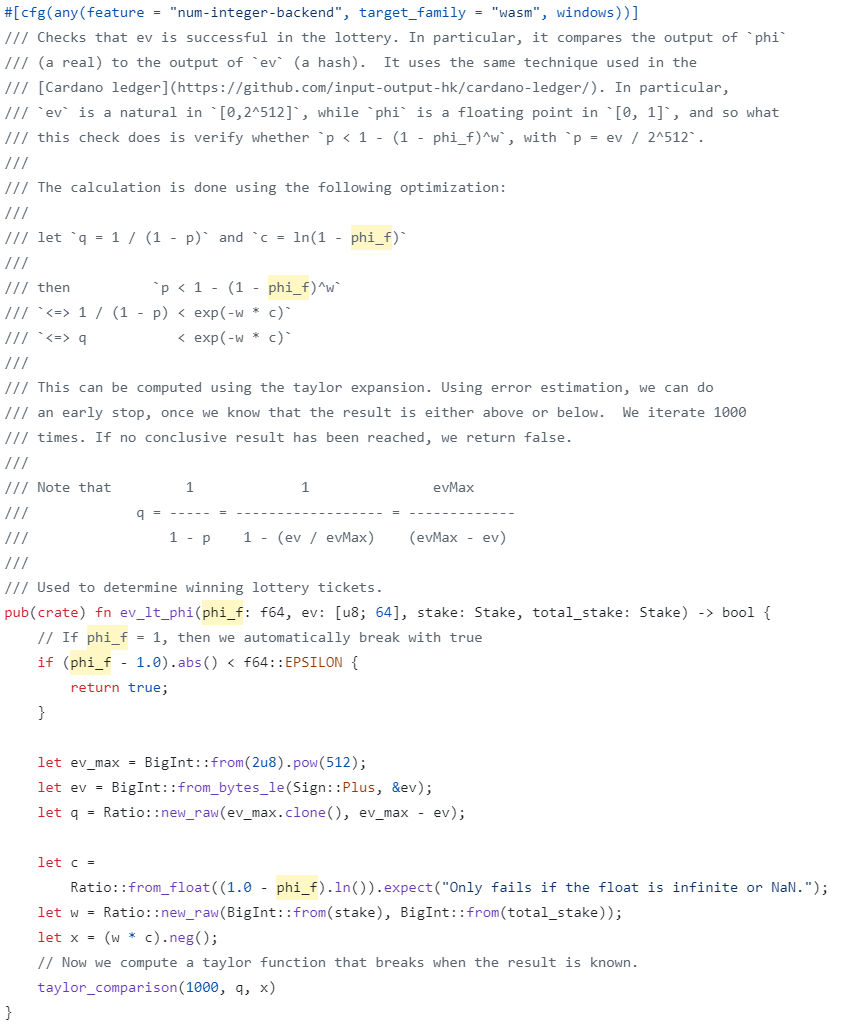
\includegraphics[width=0.9\linewidth]{mithril-ev_lt_phi-code.png}




\section{An Optimization in Mithril Paper}


There a optimization for $\phi(stake)$, and the following contents is from Mithril paper:
\\

\textit{The main outlier is the evaluation of $\phi$. Fortunately, we don’t actually need to evaluate $\phi$ in the proof: we can replace stake in the tree with $\phi(stake)$ and proceed with the comparison directly. This gives us a circuit size of $O(klogq)$, and verifier complexity of $O(\frac{klog^4q}{log(klogq)})$ as verification is dominated by a multiexponentiation based on the circuit size.}\\
\\
Which means that our benchmark results is also valid for this optimized solution, because we generated the $\mathsf{stake_i}$ randomly.




\end{document}
